\chapter{Random Walks}\label{ran_process_chap}

\term{Random Walks} are used to model situations in which an object
moves in a sequence of steps in randomly chosen directions.  Many
phenomenoa can be modeled as a random walk and we will see several
examples in this chapter.  Among other things, we'll see why it is
rare that you leave the casino with more money than you entered with
and we'll see how the Google search engine uses random walks through
the graph of the world-wide web links to determine the relative
importance of websites.


\section{A Bug's Life}

There is a small flea named Stencil.  To his right, there is an
endless flat plateau.  One inch to his left is the Cliff of Doom,
which drops to a raging sea filled with flea-eating monsters.
%
\begin{center}
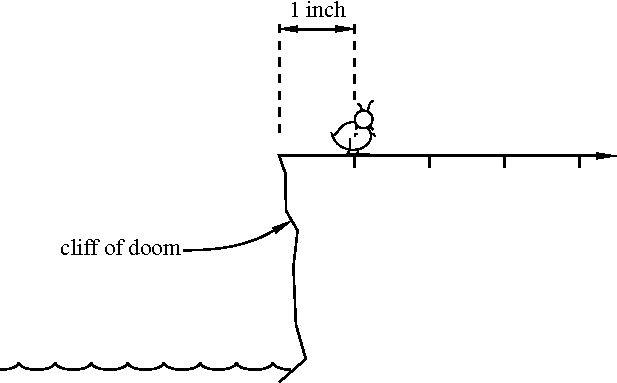
\includegraphics{stencil1}
\end{center}

Each second, Stencil hops 1 inch to the right or 1 inch to the left
with equal probability, independent of the direction of all previous
hops.  If he ever lands on the very edge of the cliff, then he teeters
over and falls into the sea.
%
\begin{center}
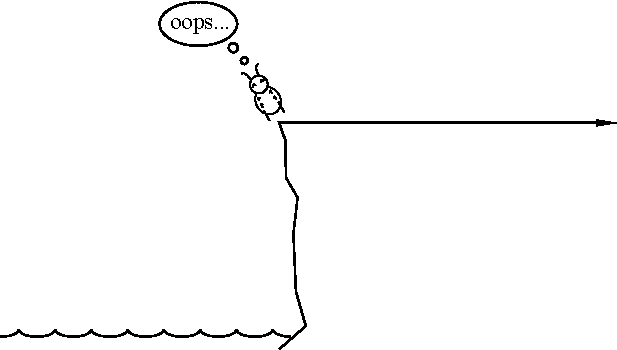
\includegraphics{stencil2}
\end{center}
%
So, for example, if Stencil's first hop is to the left, he's fishbait.
On the other hand, if his first few hops are to the right, then he may
bounce around happily on the plateau for quite some time.

Our job is to analyze the life of Stencil.  Does he have any chance of
avoiding a fatal plunge?  If not, how long will he hop around before
he takes the plunge?

Stencil's movement is an example of a \term{random walk}.  A typical
random walk involves some value that randomly wavers up and down over
time.  Many natural phenomona are nicely modeled by random walks.
However, for some reason, they are traditionally discussed in the
context of some social vice.  For example, the value is often regarded
as the position of a drunkard who randomly staggers left, staggers
right, or just wobbles in place during each time step.  Or the value
is the wealth of a gambler who is continually winning and losing bets.
So discussing random walks in terms of fleas is actually sort of
elevating the discourse.

\subsection{A Simpler Problem}

Let's begin with a simpler problem.  Suppose that Stencil is on a
small island; now, not only is the Cliff of Doom 1 inch to his left,
but also there is a Cliff of Disaster 2 inches to his right!
%
\begin{center}
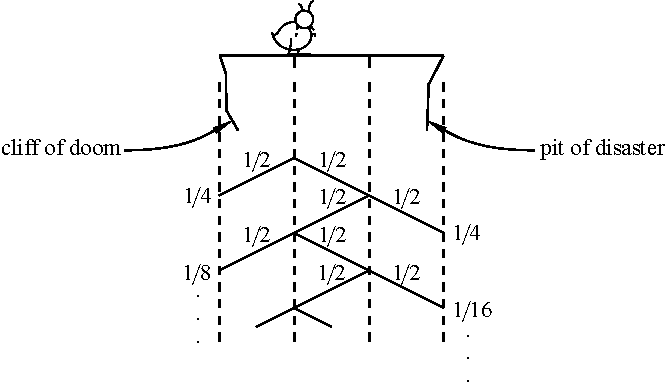
\includegraphics{stencil3}
\end{center}
%
Below the figure, we've worked out a tree diagram for his possible
fates.  In particular, he falls off the Cliff of Doom on the left side
with probability:
%
\begin{align*}
\frac{1}{2} + \frac{1}{8} + \frac{1}{32} + \ldots
    & = \frac{1}{2} \paren{1 + \frac{1}{4} + \frac{1}{16} + \ldots} \\
    & = \frac{1}{2} \cdot \frac{1}{1 - 1/4} \\
    & = \frac{2}{3}
\end{align*}
%
Similarly, he falls off the Cliff of Disaster on the right side with
probability:
%
\[
\frac{1}{4} + \frac{1}{16} + \frac{1}{64} + \ldots = \frac{1}{3}
\]
%
There is a remaining possibility: he \textit{could} hop back and forth
in the middle of the table forever.  However, we've already identified
two disjoint events with probabilities $2/3$ and $1/3$, so this happy
alternative must have probability 0.

\subsection{A Big Island}

Putting Stencil on such a tiny island was sort of cruel.  Sure, he's
probably carrying bubonic plague, but there's no reason to pick on the
little fella.  So suppose that we instead place him $n$ inches from
the left side of an island $w$ inches across:
%
\begin{center}
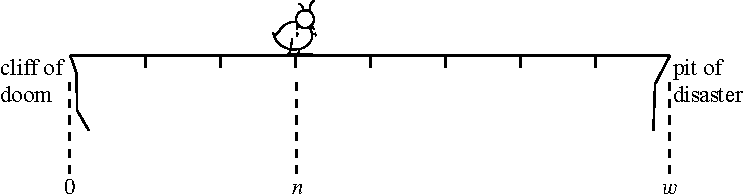
\includegraphics{stencil4}
\end{center}
%
In other words, Stencil starts at position $n$ and there are cliffs at
positions 0 and $w$.

Now he has three possible fates: he could fall off the Cliff of Doom,
fall off the Cliff of Disaster, or hop around on the island forever.
We could compute the probabilities of these three events with a
horrific summation, but fortunately there's a far easier method: we
can use a linear recurrence.

Let $R_n$ be the probability that Stencil falls to the right off the
Cliff of Disaster, given that he starts at position $n$.  In a couple
special cases, the value of $R_n$ is easy to determine.  If he starts
at position $w$, he falls from the Cliff of Disaster immediately, so
$R_w = 1$.  On the other hand, if he starts at position $0$, then he
falls from the Cliff of Doom immediately, so $R_0 = 0$.

Now suppose that our frolicking friend starts somewhere in the middle
of the island; that is, $0 < n < w$.  Then we can break the analysis
of his fate into two cases based on the direction of his first hop:
%
\begin{itemize}

\item If his first hop is to the left, then he lands at position $n-1$
and eventually falls off the Cliff of Disaster with probability
$R_{n-1}$.

\item On the other hand, if his first hop is to the right, then he
lands at position $n+1$ and eventually falls off the Cliff of Disaster
with probability $R_{n+1}$.

\end{itemize}
%
Therefore, by the Total Probability Theorem, we have:
%
\[
R_n = \frac{1}{2} R_{n-1} + \frac{1}{2} R_{n+1}
\]

\subsubsection*{A Recurrence Solution}

Let's assemble all our observations about $R_n$, the probability that
Stencil falls from the Cliff of Disaster if he starts at position $n$:
%
\[
\begin{array}{rl}
R_0 & = 1 \\
R_w & = 0 \\
R_n & = \frac{1}{2} R_{n-1} + \frac{1}{2} R_{n+1} \qquad (0 < n < w)
\end{array}
\]
%
This is just a linear recurrence--- and we know how to solve those!
Uh, right?  (We've attached a quick reference guide to be on the safe
side.)

There is one unusual complication: in a normal recurrence, $R_n$ is
written a function of preceding terms.  In this recurrence equation,
however, $R_n$ is a function of both a preceding term ($R_{n-1}$) and
a \textit{following} term ($R_{n+1}$).  This is no big deal, however,
since we can just rearrange the terms in the recurrence equation:
%
\[
R_{n+1} = 2 R_n - R_{n-1}
\]
%
Now we're back on familiar territory.

\begin{figure}[p]
\input{on-web-or-inactive/short_guide.tex}
\end{figure}

Let's solve the recurrence.  The characteristic equation is:
%
\[
x^2 - 2 x + 1 = 0
\]
%
This equation has a double root at $x = 1$.  There is no inhomogenous
part, so the general solution has the form:
%
\[
R_n = a \cdot 1^n + b \cdot n 1^n = a + b n
\]
%
Substituting in the boundary conditions $R_0 = 0$ and $R_w = 1$ gives
two linear equations:
%
\begin{align*}
0 & = a \\
1 & = a + b w
\end{align*}
%
The solution to this system is $a = 0$, $b = 1 / w$.  Therefore, the
solution to the recurrence is:
%
\[
R_n = n / w
\]

\subsubsection*{Interpreting the Answer}

Our analysis shows that if we place Stencil $n$ inches from the left
side of an island $w$ inches across, then he falls off the right side
with probability $n / w$.  For example, if Stencil is $n = 4$ inches
from the left side of an island $w = 12$ inches across, then he falls
off the right side with probability $n / w = 4 / 12 = 1 / 3$.

We can compute the probability that he falls off the \textit{left}
side by exploiting the symmetry of the problem: the probability the
falls off the \textit{left} side starting at position $n$ is the same
as the probability that he falls of the \textit{right} side starting
at position $w - n$, which is $(w - n) / n$.

This is bad news.  The probability that Stencil eventually falls off
one cliff or the other is:
%
\[
\frac{n}{w} + \frac{w - n}{w} = 1
\]
%
There's no hope!  The probability that he hops around on the island
forever is zero.  And there's even worse news.  Let's go back to the
original problem where Stencil is 1 inch from the left edge of an
infinite plateau.  In this case, the probability that he eventually
falls into the sea is:
%
\[
\lim_{w \to \infty} \frac{w - 1}{w} = 1
\]
%
Our little friend is doomed!

Hey, you know how in the movies they often make it look like the hero
dies, but then he comes back in the end and everything turns out okay?
Well, I'm not sayin' anything, just pointing that out.

%%%%%%%%%%%%%%%%%%%%%%%%%%%%%%%%%%%%%%%%%%%%%%%%%%%%%%%%%%%%%%%%%%%%%%%%%%%%%%%

\subsection{Life Expectancy}

On the bright side, Stencil may get to hop around for a while before
he sinks beneath the waves.  Let's use the same setup as before, where
he starts out $n$ inches from the left side of an island $w$ inches
across:
%
\begin{center}
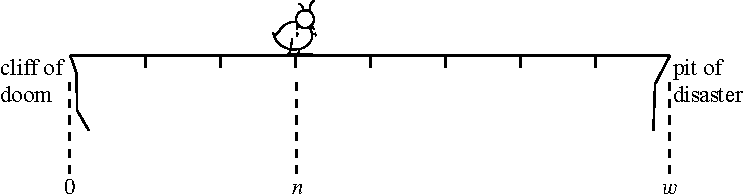
\includegraphics{stencil4}
\end{center}
%
What is the expected number of hops he takes before falling off a cliff?

Let $X_n$ be his expected lifespan, measured in hops.  If he starts at
either edge of the island, then he dies immediately:
%
\begin{align*}
X_0 & = 0 \\
X_w & = 0
\end{align*}
%
If he starts somewhere in the middle of the island ($0 < n < w$), then
we can again break down the analysis into two cases based on his first
hop:
%
\begin{itemize}

\item If his first hop is to the left, then he lands at position $n-1$
and can expect to live for another $X_{n-1}$ steps.

\item If his first hop is to the right, then he lands at position
$n+1$ and his expected lifespan is $X_{n+1}$.

\end{itemize}
%
Thus, by the Total Expectation Theorem and linearity, his expected
lifespan is:
%
\begin{align*}
X_n & = 1 + \frac{1}{2} X_{n-1} + \frac{1}{2} X_{n+1}
\end{align*}
%
The leading $1$ accounts for his first hop.

\subsubsection*{Solving the Recurrence}

Once again, Stencil's fate hinges on a recurrence equation:
%
\[
\begin{array}{rl}
X_0 & = 0 \\
X_w & = 0 \\
X_n & = 1 + \frac{1}{2} X_{n-1} + \frac{1}{2} X_{n+1} \qquad (0 < n < w)
\end{array}
\]
%
We can rewrite the last line as:
%
\[
X_{n+1} = 2 X_n - X_{n-1} - 2
\]
%
As before, the characteristic equation is:
%
\[
x^2 - 2 x + 1 = 0
\]
%
There is a double-root at 1, so the homogenous solution has the form:
%
\[
X_n = a + b n
\]
%
There's an inhomogenous term, so we also need to find a particular
solution.  Since this term is a constant, we should try a particular
solution of the form $X_n = c$ and then try $X_n = c + d n$ and then
$X_n = c + d n + e n^2$ and so forth.  As it turns out, the first two
possibilities don't work, but the third does.  Substituting in this
guess gives:
%
\begin{align*}
X_{n+1} & = 2 X_n - X_{n-1} - 2 \\
c + d(n+1) + e(n+1)^2 & = 2 (c + dn + en^2) - (c + d(n-1) + e(n-1)^2 - 2 \\
e & = -1
\end{align*}
%
All the $c$ and $d$ terms cancel, so $X_n = c + d n - n^2$ is a
particular solution for all $c$ and $d$.  For simplicity, let's take
$c = d = 0$.  Thus, our particular solution is $X_n = - n^2$.

Adding the homogenous and particular solutions gives the general form
of the solution:
%
\begin{align*}
X_n & = a + b n - n^2
\end{align*}
%
Substituting in the boundary conditions $X_0 = 0$ and $X_w = 0$ gives
two linear equations:
%
\begin{align*}
0 & = a \\
0 & = a + b w - w^2
\end{align*}
%
The solution to this system is $a = 0$ and $b = w$.  Therefore, the
solution to the recurrence equation is:
%
\[
X_n = w n - n^2 = n (w - n)
\]

\subsubsection*{Interpreting the Solution}

Stencil's expected lifespan is $X_n = n (w - n)$, which is the
\textit{product} of the distances to the two cliffs.  Thus, for
example, if he's 4 inches from the left cliff and 8 inches from the
right cliff, then his expected lifespan is $4 \cdot 8 = 32$.

Let's return to the original problem where Stencil has the Cliff of
Doom 1 inch to his left and an infinite plateau to this right.  (Also,
cue the ``hero returns'' theme music.)  In this case, his expected
lifespan is:
%
\[
\lim_{w \to \infty} 1 (w - 1) = \infty
\]
%
\textit{Yes, Stencil is certain to eventually fall off the cliff into
the sea--- but his expected lifespan is infinite!}  This sounds almost
like a contradiction, but both answers are correct!

Here's an informal explanation.  The probability that Stencil falls
from the Cliff of Doom on the $k$-th step is approximately $1 /
k^{3/2}$.  Thus, the probability that he falls eventually is:
%
\[
\pr{\text{falls off cliff}} \approx \sum_{k=1}^{\infty} \frac{1}{k^{3/2}}
\]
%
You can verify by integration that this sum converges.  The exact sum
actually converges to 1.  On the other hand, the expected time until
he falls is:
%
\[
\ex{\text{hops until fall}} \approx \sum_{k=1}^{\infty} k \cdot \frac{1}{k^{3/2}} = \sum_{k=1}^{\infty} \frac{1}{\sqrt{k}}
\]
%
And you can verify by integration that this sum diverges.  So our
answers are compatible!

%%%%%%%%%%%%%%%%%%%%%%%%%%%%%%%%%%%%%%%%%%%%%%%%%%%%%%%%%%%%%%%%%%%%%%%%%%%%%%%

\section{The Gambler's Ruin}

We took the high road for a while, but now let's discuss random walks
in more conventional terms.  A gambler goes to Las Vegas with $n$
dollars in her pocket.  Her plan is to make only \$1 bets on red or
black in roulette, each of which she'll win with probability $9/19
\approx 0.473$.  She'll play until she's either broke or up \$100.
What's the probability that she goes home a winner?

This is similar to the flea problem.  The gambler's wealth goes up and
down randomly, just like the Stencil's position.  Going broke is
analogous to falling off the Cliff of Doom and winning \$100
corresponds to falling off the Cliff of Disaster.  In fact, the only
substantive difference is that the gambler's wealth is slightly more
likely to go down than up, whereas Stencil was equally likely to hop
left or right.

We determined the flea usually falls off the nearest cliff.  So we
might expect that the gambler can improve her odds of going up \$100
before going bankrupt by bringing more money to Vegas.  But here's
some actual data:
%
\[
\begin{array}{c@{\qquad}c}
\text{$n =$ starting wealth} &
\text{probability she reaches $n + \$100$ before \$0} \\[0.5ex]
\$100 & \text{1 in 3764\underline{9}.619496\ldots} \\[0.5ex]
\$1000 & \text{1 in 37648.619496\ldots} \\[0.5ex]
\$1,000,000,000 & \text{1 in 37648.619496\ldots}
\end{array}
\]
%
Except on the very low end, the amount of money she brings makes
almost no difference!  (The fact that only one digit changes from the
first case to the second is a peripheral bit of bizarreness that we'll
leave in your hands.)

\subsection{Finding a Recurrence}

We can approach the gambling problem the same way we studied the life
of Stencil.  Supose that the gambler starts with $n$ dollars.  She
wins each bet with probability $p$ and plays until she either goes
bankrupt or has $w \geq n$ dollars in her pocket.  (To be clear, $w$
is the total amount of money she wants to end up with, not the amount
by which she wants to increase her wealth.)  Our objective is to
compute $R_n$, the probability that she goes home a winner.

As usual, we begin by identifying some boundary conditions.  If she
starts with no money, then she's bankrupt immediately so $R_0 = 0$.
On the other hand, if she starts with $w$ dollars, then she's an
instant winner, so $R_w = 1$.

Now we divide the analysis of the general situation into two cases
based on the outcome of her first bet:
%
\begin{itemize}

\item She wins her first bet with probabilty $p$.  She then has $n +
1$ dollars and probability $R_{n+1}$ of reaching her goal of $w$
dollars.

\item She loses her first bet with probability $1-p$.  This leaves her
with $n - 1$ dollars and probability $R_{n-1}$ of reaching her goal.

\end{itemize}
%
Plugging these facts into the Total Probability Theorem gives the
equation:
%
\[
R_n = p R_{n+1} + (1 - p) R_{n-1}
\]

\subsection{Solving the Recurrence}

We now have a recurrence for $R_n$, the probability that the gambler
reaches her goal of $w$ dollars if she starts with $n$:
%
\begin{align*}
R_0 & = 0 \\
R_w & = 1 \\
R_n & = p R_{n+1} + (1 - p) R_{n-1} & (0 < n < w)
\end{align*}
%
The characteristic equation is:
%
\[
p x^2 - x + (1-p) = 0
\]
%
The quadratic formula gives the roots:
%
\begin{align*}
x & = \frac{1 \pm \sqrt{1 - 4 p (1-p)}}{2p} \\
  & = \frac{1 \pm \sqrt{(1-2p)^2}}{2p} \\
  & = \frac{1 \pm (1-2p)}{2p} \\
  & = \frac{1-p}{p} \text{ or } 1
\end{align*}

There's an important point lurking here.  If the gambler is equally
likely to win or lose each bet, then $p = 1/2$, and the characteristic
equation has a double root at $x = 1$.  This is the situation we
considered in the flea problem.  The double root led to a general
solution of the form:
%
\[
R_n = a + b n
\]
%
Now suppose that the gambler is \textit{not} equally likely to win or
lose each bet; that is, $p \neq 1/2$.  Then the two roots of the
characteristic equation are different, which means that the solution
has a completely different form:
%
\[
R_n = a \cdot \paren{\frac{1-p}{p}}^n + b \cdot 1^n
\]
%
In mathematical terms, this is where the flea problem and the gambler
problem take off in completely different directions: in one case we
get a linear solution and in the other we get an exponenetial
solution!

Anyway, substituting the boundary conditions into the general form of
the solution gives a system of linear equations:
%
\begin{align*}
0 & = a + b \\
1 & = a \cdot \paren{\frac{1-p}{p}}^w + b
\end{align*}
%
Solving this system, gives:
%
\begin{align*}
a & = \frac{1}{\paren{\frac{1-p}{p}}^w-1} &
b & = - \frac{1}{\paren{\frac{1-p}{p}}^w-1} &
\end{align*}
%
Substituting these values back into the general solution gives:
%
\begin{align*}
R_n
    & = \paren{\frac{1}{\paren{\frac{1-p}{p}}^w-1}} \cdot
        \paren{\frac{1-p}{p}}^n - \frac{1}{\paren{\frac{1-p}{p}}^w-1} \\
    & = \frac{\paren{\frac{1-p}{p}}^n-1}{\paren{\frac{1-p}{p}}^w-1}
\end{align*}
%
(Suddenly, Stencil's life doesn't seem so bad, huh?)

\subsection{Interpreting the Solution}

We have an answer!  If the gambler starts with $n$ dollars and wins
each bet with probability $p$, then the probability she reaches $w$
dollars before going broke is:
%
\[
\frac{\paren{\frac{1-p}{p}}^n-1}{\paren{\frac{1-p}{p}}^w-1}
\]

Let's try to make sense of this expression.  If the game is biased
against her, as with roulette, then $1-p$ (the probability she loses)
is greater than $p$ (the probability she wins).  If $n$, her starting
wealth, is also reasonably large, then both exponentiated fractions
are big numbers and the -1's don't make much difference.  Thus, her
probability of reaching $w$ dollars is very close to:
%
\[
\paren{\frac{1-p}{p}}^{n-w}
\]
%
In particular, if she is hoping to come out \$100 ahead in roulette,
then $p = 9/19$ and $w = n + 100$, so her probability of success is:
%
\[
\paren{\frac{10}{9}}^{-100} = 1 \text{ in } 37648.619496
\]
%
This explains the strange number we arrived at earlier!

\subsection{Some Intuition}

Why does the gambler's starting wealth have so little impact on her
probability of coming out ahead?  Intuitively, there are two forces at
work.  First, the gambler's wealth has random upward and downward
\textit{swings} due to runs of good and bad luck.  Second, her wealth
has a steady, downward \textit{drift} because she has a small expected
loss on every bet.  The situation is illustrated below:
%
\begin{center}
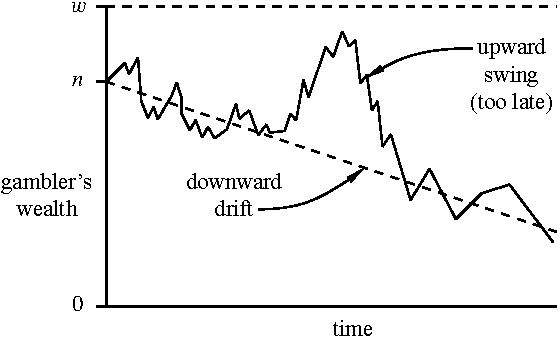
\includegraphics{gambler}
\end{center}

For example, in roulette the gambler wins a dollar with probability
$9/19$ and loses a dollar with probability $10/19$.  Therefore, her
expected return on each bet is $1 \cdot 9/10 + (-1) \cdot 10/19 = -
1/19$.  Thus, her expected wealth drifts downward by a little over 5
cents per bet.

One might think that if the gambler starts with a billion dollars,
then she will play for a long time, so at some point she should have a
lucky, upward swing that puts her \$100 ahead.  The problem is that
her capital is steadily drifting downward.  And after her capital
drifts down a few hundred dollars, she needs a huge upward swing to
save herself.  And such a huge swing is extremely improbable.  So if
she does not have a lucky, upward swing early on, she's doomed
forever.  As a rule of thumb, \textit{drift} dominates \textit{swings}
over the long term.

%%%%%%%%%%%%%%%%%%%%%%%%%%%%%%%%%%%%%%%%%%%%%%%%%%%%%%%%%%%%%%%%%%%%%%%%%%%%%%%

\section{Pass the Broccoli}

Here's a game that involves a random walk.  There are $n+1$ people,
numbered $0, 1, \ldots, n$, sitting in a circle:
%
\begin{center}
\begin{picture}(120,120)(-60,-60)
% \put(-60,-60){\framebox(120,120){}} % bounding box
\put(0.000000,50.000000){\makebox(0,0){$0$}}
\put(0.000000,36.000000){\makebox(0,0){$\mathbf{B}$}}
\put(23.236159,44.272801){\makebox(0,0){$1$}}
\put(41.149193,28.403237){\makebox(0,0){$2$}}
\put(49.635444,6.026834){\makebox(0,0){$3$}}
\put(46.750812,-17.730244){\makebox(0,0){$\cdot$}}
\put(33.156133,-37.425537){\makebox(0,0){$\cdot$}}
\put(11.965783,-48.547091){\makebox(0,0){$k-1$}}
\put(-11.965783,-48.547091){\makebox(0,0){$k$}}
\put(-33.156133,-37.425537){\makebox(0,0){$k+1$}}
\put(-46.750812,-17.730244){\makebox(0,0){$\cdot$}}
\put(-49.635444,6.026834){\makebox(0,0){$\cdot$}}
\put(-41.149193,28.403237){\makebox(0,0){$n-1$}}
\put(-23.236159,44.272801){\makebox(0,0){$n$}}
\end{picture}
\end{center}
%
The B indicates that person 0 has a big stalk of nutritious broccoli,
which provides 250\% of the US recommended daily allowance of vitamin
C and is also a good source of vitamin A and iron.  (Typical for a
random walk problem, this game orginally involved a pitcher of beer
instead of a broccoli.  We're taking the high road again.)

Person 0 passes the broccoli either to the person on his left or the
person on his right with equal probability.  Then, that person also
passes the broccoli left or right at random and so on.  After a while,
everyone in an arc of the circle has touched the broccoli and everyone
outside that arc has not.  Eventually, the arc grows until all but one
person has touched the broccoli.  That final person is declared the
winner and gets to keep the broccoli!

Suppose that you allowed to position yourself anywhere in the circle.
Where should you stand in order to maxmize the probability that you
win?  You shouldn't be person 0; you can't win in that position.  The
answer is ``intuitively obvious'': you should stand as far as possible
from person 0 at position $n / 2$.

Let's verify this intuition.  Suppose that you stand at position $k
\neq 0$.  At some point, the broccoli is going to end up in the hands
of one of your neighbors.  This has to happen eventually; the game
can't end until at least one of them touches it.  Let's say that
person $k - 1$ gets the broccoli first.  Now let's cut the circle
between yourself and your other neighbor, person $k+1$:
%
\[
\begin{array}{cccccccccccccc}
k & (k-1) & \ldots & 3 & 2 & 1 & 0 & n & (n-1) & \ldots & (k+1) \\
  & \mathbf{B} \\
\end{array}
\]
%
Now there are two possibilities.  If the broccoli reaches you before
it reaches person $k+1$, then you lose.  But if the broccoli reaches
person $k+1$ before it reaches you, then every other person has
touched the broccoli and you win!  This is just the flea problem all
over again: the probability that the broccoli hops $n-1$ people to the
right (reaching person $k+1$) before it hops 1 person to the left
(reaching you) is $1 / n$.  Therefore, our intution was compeletely
wrong: \textit{your probability of winning is $1 / n$ regardless of
where you're standing!}


\endinput
